% --------------------------------------------------------------------------- %
%      _ _                                                _       _           %
%   __| (_)_   _    __ _ _ __  _ __  _ __ ___   __ _  ___| |__   | |_ ___     %
%  / _` | | | | |  / _` | '_ \| '_ \| '__/ _ \ / _` |/ __| '_ \  | __/ _ \    %
% | (_| | | |_| | | (_| | |_) | |_) | | | (_) | (_| | (__| | | | | || (_) |   %
%  \__,_|_|\__, |  \__,_| .__/| .__/|_|  \___/ \__,_|\___|_| |_|  \__\___/    %
%          |___/        |_|   |_|                                             %
%                                                                             %
%                                                    _                        %
%                    __ _ _ __   _ __ ___  _   _ ___(_) ___                   %
%                   / _` | '__| | '_ ` _ \| | | / __| |/ __|                  %
%                  | (_| | |    | | | | | | |_| \__ \ | (__                   %
%                   \__,_|_|    |_| |_| |_|\__,_|___/_|\___|                  %
% --------------------------------------------------------------------------- %
\chapter{A DIY Approach to AR in the Sonic Arts}
\label{sec: method}
%\markboth{}{A DIY Approach to AR in the Sonic Arts}
\epigraph{\emph{Our environment is not a play, a performance in which only minor modifications are possible. It's an improvisation,[…] the nature of the interaction is radically open.}}{\citep{vermeulen2015}}

\begin{figure}
    \centering
    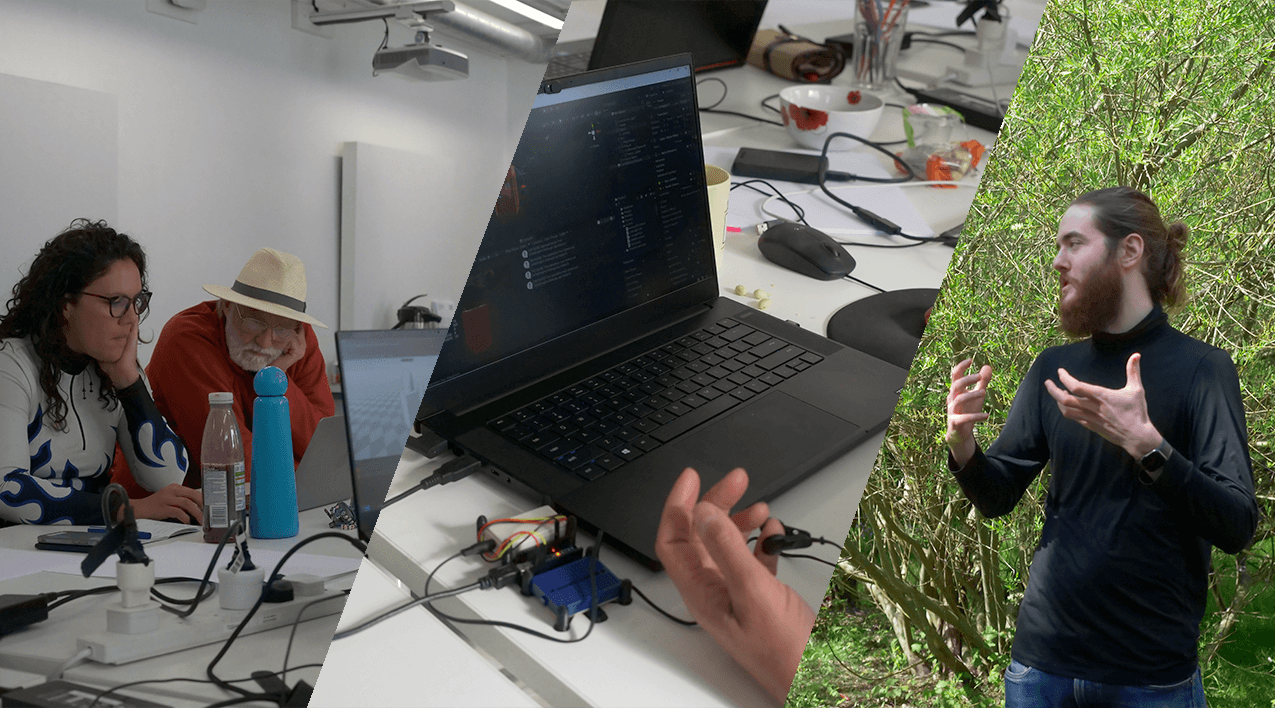
\includegraphics[width=1\linewidth]{04-method/chapter-fig.png}
    \captionsetup{labelformat=empty}
    \caption[\autoref*{sec: method}'s page-figure: Photographs from the Embodiment Hackathon at Sussex, April 30th - May 1st, (from \citeauthor{bonarjee2022}, \citeyear{bonarjee2022})]{}
\end{figure}

\clearpage
% --------------------------------------------------------------------------- %
\section{Summary}\label{sec: method-summary}
In \autoref{sec: review}, the historical origins, contextual trends, exceptions, and contemporary forms of \gls{ar} technologies were outlined. Additionally, examples of \gls{ar}'s use in the arts were provided, along with specific rationales for their use, e.g. sensory engagement, collaborative expression, and activism and agency. A positionality was established that demonstrates that \gls{ar}'s use in the arts is at odds with its origination in military and industrial applications. In the \autoref{sec: theory}, I outlined a trio of lenses through which we may begin to consider the material, embodied, and spatial aspects of sound art using \gls{ar}. In examining complex musical material, it was identified that digital musical systems or `performance ecosystems' offer us fertile conceptual ground for description of material, in the creation and evaluation of rich experiences. The work of researchers approaching experience from an enactivist perspective when working with XR technologies was then outlined. Finally, an examination of the current state of the `Metaverse' as a space to describe XR experience in general was critiqued. These three lenses all drew from an understanding of art \textit{as} experience, and the disconnection between art and everyday life, an alienation that comes as no surprise given its commodity fetishisation by free-market capitalism. Moreover, the lenses were contextualised within a 4EC approach to experience, which posits that cognitive processes are embodied, embedded, enacted and extended; inseparable from the brain-body-environment that they constitute and are situated. In the current chapter I will be outlining my methodological approach that has informed both the theoretical, and practical sides of the research: designing, performing, and evaluating sound art \gls{ar} experiences (\textit{sound \gls{art}} to borrow from Rhodes \citeyearpar{rhodes2018}). A review of the outstanding research questions will be outlined, to provide the chapter a clear direction into the ensuing three study chapters.

\begin{enumerate}
    \RQmedium
    \RQexperience
\end{enumerate}

This thesis approaches the above questions by making use of several established practice research methods. Broadly, these methods have led to practical contributions that will be explored in the following three study chapters: 
\begin{itemize}
    \item the creation and iterative design of multisensory sound ARt
    \item a set of open design patterns for creating similar sound \gls{art} compositions and performances
\end{itemize}
These practical contributions have functioned both as ongoing research probes, and as platforms for open and reproducible artistic work for the wider experimental music research community. The methods present in this thesis have stayed consistent with their original proposal, with the exception of specific methods of data collection and analysis being adapted to suit the restrictions of the COVID-19 pandemic, which commenced three months after the start of research. 

As will be developed on in \autoref{sec: discussion-patterns}, it is within this context of creating, developing, implementing and iterating on a set of open design patterns for \gls{ar} art and music that the research methods employed in the following chapters are carried out. This started with a motivation for creating smaller experiences, that were simple in their sensory modulation and instrumental reactivity, with the view to later incorporate them into larger scale interactive \gls{ar} experiences once sufficiently tested. However, due to COVID-19, the prospect of user-testing and iterating on the design of multiple experiences, especially large scale ones, through participant feedback became increasingly difficult to facilitate and plan for. Thus, I opted to focus on developing working sound art \gls{ar} prototypes that I myself would compose with regularly, tweak, and iterate upon. Then, and there, an \gls{ar} research and compositional practice began.

It is pertinent to mention that practical work, where carried out, has always been documented for analysis, open-research, and archival purposes. I found the combination of \href{https://sambilbow.github.io}{my personal website} as well as \href{https://github.com/sambilbow}{GitHub} and \href{https://youtube.com/@sambilbow}{YouTube} a suitable and cost-effective solution for this. Links to project files will be included in the study chapters, and cited websites have been archived using \rurl{archive.today} \footnote{\url{https://en.wikipedia.org/wiki/Archive.today}}. Before outlining the specific methods touched on in later chapters, I would first like to touch upon the concept of resistance, and its role in motivating the methodological approach taken in the thesis.



% --------------------------------------------------------------------------- %
\section{Resistance in Practice}\label{sec: method-resistance}
Formative in the development of the methodological approach of this thesis has been the concept of `resistance'. In short, this could be characterised as a motivation for changing or acting against the state of the art, practice, technology, or philosophy, out of a discontent for its status quo. This isn't to be confused by resistance in the sense of experiencing resistance to \textit{do} something, although as might be expected, that has reared its head a few times over the last three years too. It is difficult to place resistance into the linear narrative of this text; some resistance formed my initial motivations for the carrying out of this research, and some was garnered along the way, especially around the time of the unfortunate uptake in `Metaverse' as a term to describe the sum total of all creative XR development and labour. Either way, resistance has made up a large portion of my approach to \gls{ar} technologies, its role within digital music and humanities more broadly. These forms of resistance can be separated into three main categories.

\subsection{AR as Consumer Technology}\label{sec: method-resistance-maker}
As referred to in \autoref{sec: theory-experience}, contemporary design research in the fields of computational art and music have in recent years rallied behind the broader `free / libre and open-source software' and `open-source hardware' ethoses (abbreviated to FLOSS and OSH respectively). This approach, often hand-in-hand with the Maker, DIY, and Hardware Hacking subcultures, stands in stark contrast to the goings-on of mega-corporations board rooms, with their design `sprints', `agile' workflows, and `human (customer)-centred' design. The approaches taken by these subcultures towards embodied design and composition workflows however, has been highly beneficial for the field. In the case of digital music making, software,hardware, and live-coding tools like PureData, Maximilian, Supercollider, ixilang, Sonic Pi, TidalCycles, FluCoMa, and Bela have granted students, researchers, and composers across disciplines, free and beginner-friendly access to a wealth of software tutorials, examples, and tools for advanced real-time sampling and synthesis techniques.

It could be proposed, that this approach is motivated in part by a resistance against many of the `features' typically found in commercial `closed-source' software and hardware. Providing significant barriers to accessible learning, creativity, and artistic authenticity, these include lack of interoperability with other software, use of proprietary file formats, high initial or recurring subscription costs, and restricted access to lower-level parameters, functions, and settings. It is within this resistance against the closed-source and / or commercial that the practical work of this thesis attempts to situate itself, drawing on its implicit designerly practices and aesthetics. As a result, the path taken to address the key areas of the thesis has involved the bringing into the fore, knowledge from the creative practice of hacking, making, designing, and iterating with experimental and DIY open-source hardware and software.

While commentary on the considerable role of un(der)funded volunteer labour involved in open-source tools and projects is outside of the scope of this thesis, it is worth mentioning. In this way, `open-source' is never taken to describe the best way of carrying out a project, rather I hope to convey that the ideals and features of an open-source ethic are beneficial to the aims of this thesis, vis-à-vis developing the understanding of new technologies within the NIME field, and attempting to manoeuvre what is essentially a minefield of technologies that are only available today because of U.S. defence funding.

\subsection{AR as Visual}\label{sec: method-resistance-ocularcentrism}
A second form of resistance that the methodological approach of this thesis explored is the ocularcentrism found in \gls{ar} technologies mentioned previously in \autoref{sec: ar-sensory-visual}. As a practitioner of music, and audio related technologies, this has provided a significant portion of the motivation for carrying out the present research, as well as a significant portion of the challenges faced when attempting to develop \gls{ar} as a medium for sound-based interactive experiences. Developing new interfaces for musical expression invariably leads to the appropriation of technology `not meant' or `not for' musical expression, and this is where NIME practice has considerable crossover into the maker / DIY / hardware-hacking subculture. The present thesis approaches ocularcentrism head-on, not through replacing the visual, but through re-ordering, with the aim to even-out, the sensory hierarchy of \gls{ar} technologies. 

Realistically, however, technologies relating to touch, and especially the chemical senses, present significant barriers compared to the visual and auditory senses in terms of access, cost, expertise, and time. In this research I have attempted to make room for future cases where this technology may be available, by using open-source software and hardware where possible, and by presenting a case for the design of multisensory \gls{ar} experience in the set of design patterns in \autoref{sec: discussion-patterns}. Thus, the present thesis approaches audiovisual, gestural \gls{ar} as a starting point for my own \gls{ar} composition and performance, with a mindful eye (or ear) to the future capabilities of multisensory HCI technologies.

\subsection{AR as Overlay}\label{sec: method-resistance-overlay}
The third form of resistance drawn from in the thesis is that of \gls{ar}'s paradigmatic function as an `overlay' device. So far, the origin of this approach, and contemporary alternatives to it have been explored \autoref{sec: ar-process}, with a case being made by practitioners \citep{mann1994,schraffenberger2018,chevalier2020} towards re-situating \gls{ar} as a process of perceptual mediation. In the present research, the resistance towards \gls{ar} functioning as a `heads-up display' (HUD) has led to propositions on how these approaches intersect with a `4E's' approach to cognition, later on, in \autoref{sec: discussion-medium-embodiment}. In practice, it has motivated the \gls{ar} experiences developed in this research to go beyond passively layering sensory stimuli in front of immersants \textit{as experience itself}. This is achieved by presenting experiences that are contingent on immersant movement, gesture, and environmental sounds, not only passive viewership. In this way, the \gls{ar} experience can be thought more of as a hybridisation or alteration of reality rather than an simple `HUD' augmentation of reality.

As with multisensory technologies though, technologically achieved `diminished reality' and other non-augmenting subforms are, in general, more computationally expensive and beyond the scope of the research practice due to lack of expertise and time. By way of acknowledging their importance as valid methods of perceptual mediation, they are accounted for in the design patterns presented in \autoref{sec: discussion-patterns}.



% --------------------------------------------------------------------------- %
\section{Research in Practice}
The three ensuing chapters, \textit{\nameref{sec: area} (2020)}, \textit{\nameref{sec: polaris} (2021)}, and \textit{\nameref{sec: polygons} (2022)} outline and analyse three \gls{ar} interactive music systems developed over the course of this thesis, each with different but converging focuses. They make up practical contributions to knowledge, as well as forming the grounds for the propositions in \autoref{sec: discussion-medium}. Though they were initially guided by a loose set of proto-design patterns \citep{bilbow2020}, it is through the insights and analysis gained in their creation and iteration that the \nameref{sec: discussion-patterns} in \autoref{sec: discussion} have been developed; they can therefore also be thought of as research probes in their own right.

\textit{area\textasciitilde{}} was the starting point for practical work in the present thesis. It is a non-visual audio \gls{ar} experience centred around the self-composition of a hybrid listening environment using an ambisonic microphone, head-, and hand-tracking. As will be expanded upon in the next chapter, due to the circumstances of the COVID-19 lockdown, I opted for an autobiographical design method for the iteration and evaluation of the system. Out of the evaluation of this project, namely the endeavour to expand into audiovisual \gls{ar} experiences, I discovered a suitable platform the develop the rest of doctoral research on: the open-source Project North Star \gls{ar} headset. \textit{polaris\textasciitilde{}} describes an \gls{ar} experience that was developed to examine the suitability of the Project North Star \gls{ar} headset's use in an audiovisual installation context. Participant studies were conducted and an evaluation of their experience was carried out via the grounded theory method of analysis. \textit{polygons\textasciitilde{}} was a direct result of sharing the experience of artistic \gls{ar} with the participants of \textit{polaris\textasciitilde{}}. In proposing an Sound ARt Performance Practice, it describes the composition of a set of \gls{ar} musical instruments, technical setup, and considerations of deploying an \gls{ar} headset as a medium for musical performance.


% --------------------------------------------------------------------------- %
\section{NIME'22 Ethics Statement}\label{sec: polaris-ethics}
The study followed University of Sussex ethics guidelines approved by the Social Sciences \& Arts Cross-Schools Research Ethics Committee with the reference code: ER/SMB44/3.

\subsection{Socio-economic Fairness}\label{sec: polaris-ethics-}
At all stages of this research, I have sought to minimise the outlay required to invest in technology needed to implement \textit{polaris\textasciitilde{}}. This has meant opting for FLOSS (free / libre open-source software) where possible: The software companion to the North Star, Project Esky \footnote{`Esky' is a colloquial term for an ice-cooler in Australia, etymologically deriving from the word `Eskimo'. I acknowledge the use of this term as being pejorative towards the indigenous populations of the Greenlandic and Canadian Inuit, Alaskan Iñupiat, and Yupik peoples; fully recognise their human and land rights, and have made the effort to redact the word within the main body of this article.}, PureData, and OBS. Ideally the 3D-engine used would also be FLOSS, i.e. Godot, but due to time constraints I have opted for Unity which I am already experienced with, and which has great documentation and free learning materials.

Though the Project North Star headset is OSH (open-source hardware), I have not had time to develop DIY and OSH audio solution yet, but any bluetooth bone-conduction headphones are compatible.

Unfortunately, the \textit{polaris\textasciitilde{}} experience (and as such, its framework) is not compatible with macOS and Linux, although it will be once Ultraleap provide their V5 drivers for hand-tracking on those operating systems.

It is worth noting that, as with most smaller suppliers of technology, the current global chip shortage has made getting hold of some components quite difficult at times, and recently the developers of the display driver board had to take the time to redesign it to get around this; the headset was not available to buy new for several months during this period. I suppose that this points to an issue: \textit{`accessibility'} doesn't always correlate with \textit{`availability'}, especially when trying to circumvent expensive consumer technologies.

Since beginning these studies, Intel has discontinued their T261/T265 range of products, meaning that anyone looking to build the headset today would have difficulty including movement tracking, a fairly essential component of effective \gls{ar} experiences. I am fully aware of the roadblock this puts in the way of \textit{polaris\textasciitilde{}} currently being reproducible as per its framework, but thankfully efforts are underway by developers in the community to solve this issue by migrating to Luxonis' modular and open-source range of tracking cameras; leaving the proprietary and closed-source hardware and software of Intel behind. If anything, their announcement has served as a reminder of the importance of FOSS/H components in community-led projects.

\subsubsection{A note on the environment}\label{sec: polaris-ethics-environment}
While it is certainly difficult to mitigate the environmental impact entirely from projects that rely on technology, I have opted for compostable PLA material for the construction of the headset used in the study to reduce e-waste in the event of breakage or updates to the hardware design.

\subsection{Study Participants}\label{sec: polaris-ethics-participants}
\subsubsection{Accessibility}\label{sec: polaris-ethics-accessibility}
In anticipating the possibility of a diverse set of accessibility needs, I provided stepped and step-free access instructions to get to the lab, maintained clearly formatted correspondence with participants via e-mail, and observed the university's COVID-19 policy during the study. Participants wearing glasses were able to use the headset with or without their glasses, and the volume of the \gls{ar} scene was kept at a tolerable level, with the option given to participants to increase or decrease it.

\subsubsection{Inclusion}\label{sec: polaris-ethics-inclusion}
Participants were recruited via internal University undergraduate and postgraduate mailing lists and were selected to ensure a diverse cohort of individuals from differing ethnicities, genders, and ages.

\subsubsection{Remuneration}\label{sec: polaris-ethics-renumeration}
Study participants were compensated £15 each for the 45 minutes - 1 hour in which they took part in the study.

\subsubsection{Consent}\label{sec: polaris-ethics-consent}
All participants provided written consent to take part in the questionnaire, experience, and interview; and also to being video and audio recorded during this time. They could at any time choose not to participate further, without being penalised or disadvantaged in any way. Their involvement in the study did not in any way impact their marks, assessments, or future studies. After analysis, their transcribed contributions were approved, and they had the opportunity to remove any anonymous, but still sensitive information.

\subsubsection{Data and privacy}\label{sec: polaris-ethics-data}
Data from the studies: video and audio recordings, transcriptions, and analysis files are secured on a separate hard drive and are password protected. All quotes and data have been anonymised in accordance with data protection legislation.



% --------------------------------------------------------------------------- %